% !TeX encoding = UTF-8
%% (requires IEEEtran.cls version 1.7 or later) with an IEEE conference paper.
\documentclass[article]{IEEEtran}

\renewcommand\IEEEkeywordsname{Keywords}

\pagenumbering{gobble}

\usepackage[utf8]{inputenc}

% *** GRAPHICS RELATED PACKAGES ***
%\usepackage[pdftex]{graphicx}
\usepackage{graphicx}
%\usepackage[dvips]{graphicx}
% to place figures on a fixed position
\usepackage{float}

% *** PDF, URL AND HYPERLINK PACKAGES ***
\usepackage{url}

% correct bad hyphenation here
\hyphenation{NetFPGA}

\usepackage{xcolor}



% \renewcommand\note[1]{} % uncomment this line to hide notes

%%%%%%%%%%%%%%%%%%%%%%%%%%%%%%%%%%%%%%%%%%%%%%%%%%%
%%%%%%%%%%%%%%%%%%%%%%%%%%%%%%%%%%%%%%%%%%%%%%%%%%%
%%%%%%%%%%%%%%%%%%%%%%%%%%%%%%%%%%%%%%%%%%%%%%%%%%%
%


% LaTeX quick ref
%
% \cite{refname} to place citation
%
% \label{label_name} to place a label, which can be reference by \ref{label_name}
%
% new paragraph -> empty line between text
%
% \noindent to not indent paragraphs first line
%
% create list with : \begin{itemize} \end{itemize}
% \begin{itemize
% \renewcommand to renew numbering \labelitemi{--} to select bullet type
% \item item elem 1
% \item item elem2
% \end{itemize}
%
% et alia (et al.) should be emphasized (i.e in italic) with \emph{et al.}
%
% to add figure, htb is placement selector , !overrid internal paramters
%\begin{figure}[!htb]
%    \centering
%    \includegraphics[width=0.5\textwidth]{FIG.png}
%    \caption{Caption}
%    \label{fig:label}
%\end{figure}
%
% ~ concatenates dynamic text with literals
%
% long dash is --
%
% `is single quoted' , ``is double qouted"
%
% to autoformat with latexindent: latexindent -w  -m -l defaultSettings.yaml ProtoImplFPGA.tex


\begin{document}
% conference papers do not typically use \thanks and this command
% is locked out in conference mode. If really needed, such as for
% the acknowledgment of grants, issue a \IEEEoverridecommandlockouts
% after \documentclass
% paper title
% can use linebreaks \\ within to get better formatting as desired
\title{Time synchronization solution for FPGA based distributed Network Monitoring}
%\titleheader{25th Telecommunications forum TELFOR 2017 \hfill Serbia, Belgrade, November 21-22, 2017.}

% author names and affiliations
% use a multiple column layout for up to three different
% affiliations
\author{Ferenc Nándor Janky} %\thanks{Ferenc Nándor Janky	is with the Department of \mbox{Telecommunications} and
%        \mbox{MediaInformatics},
%        Faculty of Electrical Engineering and Informatics, Budapest University of Technology and \mbox{Economics},
%        Magyar tudósok
%        körútja 2., 1117 Budapest, Hungary (\mbox{phone: +36704213213}; \mbox{e-mail:
%            fecjanky@gmail.com})}%
%}%

%\markboth{25th Telecommunications forum TELFOR 2017 \hfill Serbia, Belgrade, November 21-22,
%    2017.}%
%{}

%\IEEEpubid{\makebox[\columnwidth]{978-1-5386-3073-0/17/\$31.00~\copyright~2017 IEEE\hfill}
%    \hspace{\columnsep}\makebox[\columnwidth]{ }}

% make the title area
\maketitle

\begin{abstract}
    \boldmath
    TODO(Pali)
\end{abstract}

\begin{IEEEkeywords}
    FPGA, Networking, Protocol stack, VHDL
\end{IEEEkeywords}

% no keywords
\section{Introduction}\label{sec:Intro}

TODO(Pali): 1.oldal

\section{Challenges and Requirements in detail}\label{sec:Challanges}

%TODO(Fec) : 0.5 oldal
%- Monotonic clock
%- Remote locations, skewing clock
%- Adaptation to legacy systems 
%- Precision requirements (Fendler Tomi TDK)

For a distributed monitoring solution described in Section~\ref{sec:Intro} there is a strong requirement for having
a monotonic clock -- otherwise even with a single monitoring node packet reordering would happen if those are inspected
based on their timestamps as a consequence the need for monotonic system time is inherent. 

Another challenge comes from the fact that a distributed monitoring system has its components geographically
separated from each other therefore the clock frequency and the time information of the clocks of the nodes have to be 
frequency and phase synchronized to each other with some given threshold. This problem has many solutions e.g. using GPS based synchronization 
systems~\cite{GPS-CLOCK} that requires additional installation expenditures on an indoor site that has no installed 
antenna system to carry the GPS signal inside the building and could also result in extensive cabling work. 
A convenient alternative for this is to use network time synchronization that uses a telecommunication network for
exchanging packets as per a specified protocol to achieve frequency and phase synchronization. Examples for this
are Network Time Protocol (NTP)~\cite{NTP} and Precision Time Protocol (PTP)~\cite{PTP}.

When speaking about time synchronization the following properties describe a clock:
\begin{itemize}
	\item accuracy -- \emph{i.e.} how good is the time information compared to some reference
	\item precision -- \emph{i.e.} how precise is a tick of the clock compared to some reference
	\item stability -- \emph{i.e.} how does the clock frequency change  e.g over time or based on external temperature changes etc.
\end{itemize} 

The biggest challenge of all -- as usual -- is to adapt to the existing monitoring framework described in \ref{sec:SGA-Monitoring} 
in with minimal modification to the existing solution while satisfying all the precision and accuracy related requirements. 
This framework is built from FPGA based monitoring cards that are capable of capturing on high-speed network interfaces --
with fine-grained time-stamping capabilities -- that has their own existing time-keeping facilities. 
The approach was to provide a new FPGA based card that implements these functions:
\begin{itemize}
	\item network time synchronization
	\item local time synchronization
	\item interfacing with the existing nodes -- OAMP functionalities
\end{itemize}

\section{Related Work}

\subsection{Network Monitoring}
TODO(Pali): 1.oldal


\subsection{FPGA based packet processing}
 TODO(Pali): 1.oldal

\IEEEpubidadjcol

\section{Architecture of the distributed time synchronized monitoring system}

\subsection{Generic concept}
For providing easy adaptation into the existing system and also taking into account FPGA resource usage a hybrid solution
has been designed that implements network time synchronization on a standalone card that distributes the digital timing 
information over a dedicated control bus as illustrated by Figure~\ref{fig:concept}. 
The synchronization framework provides a platform independent agent that 
can be integrated into the existing cards' top level modules and used through a well defined and portable interface. 
The agent itself has less complexity as a result the solution does not waste CLB resources as if the whole network 
synchronization stack were instantiated N times on all monitoring node cards also resulting in better internal synchronization
compared to the replicated stacks as those can have skew to each other within the boundaries as specified by their protocol.

\begin{figure}[!htb]
    \centering
    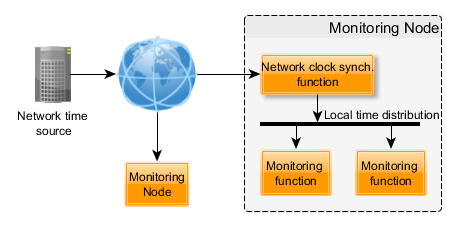
\includegraphics[width=0.45\textwidth]{figures_raw/concept.png}
    \caption{Conceptual model of distributed monitoring framework}
    \label{fig:concept}
\end{figure}

As seen on Figure~\ref{fig:concept} each node has it's own network synchronization function therefore the accuracy and
precision between two monitoring nodes can be guaranteed only to an extent that the utilized time synchronization
protocol provides. This is in the magnitude of milliseconds of a software implementation of NTP -- however with FPGA based implementation
this precision can be increased --  and in the magnitude of
microseconds or nanoseconds depending on the PTP version used and also on the underlying network.
The key concept is that over the local time distribution bus even greater synchronicity can be achieved as there is less
perturbation between the HW implementations of the transmitting and receiving ends -- no OS scheduler, no network \emph{etc.} --
and also frequency synchronization can be easily achieved by implementing a synchronous bus -- \emph{i.e.} transmitting the
clock signal along with the data.

\subsection{External time synch. subsystem}
TODO(Fec) : 0.5 oldal PTP vs. NTP ( PTP requires network capabilities)
keywords: NTP vs. PTPv1, PTPv2 network reliance, selection of NTP consideration

\subsection{Internal time synch. subsystem}
TODO(Fec) : 0.5 oldal
 \begin{itemize}
 	\item draw figure on closed loop control 
 	\item describe the figure
 	\item deduce the theoretical precision of that
 \end{itemize}

\section{Implementation details}

- Clock card intro 
- parameters briefly

\subsection{External time synch. subsystem}
TODO(Fec) : 0.5 oldal
 \begin{itemize}
 	\item refer to ProtoImpl
 	\item add NTP module figure
 	\item describe parts
 \end{itemize}

\subsection{Internal time synch. subsystem}
TODO(Fec) : 0.5 oldal
- describe HiSTI

\section{Verification \& Results}

TODO(Fec) : 1.5 oldal

- Describe the verification method in detail
- Matlab graph, long-term vs. short-term 


\section{Conclusion}

TODO(Fec \& Pali): 0.5 oldal


References: 0.5 oldal

% http://www.ctan.org/tex-archive/biblio/bibtex/contrib/doc/
% The IEEEtran BibTeX style support page is at:
% http://www.michaelshell.org/tex/ieeetran/bibtex/

%\bibliographystyle{IEEEtran}
% argument is your BibTeX string definitions and bibliography database(s)
%\bibliography{references}

%
% <OR> manually copy in the resultant .bbl file
% set second argument of \begin to the number of references
% (used to reserve space for the reference number labels box)

%\begin{thebibliography}{1}
%
%\bibitem{IEEEhowto:kopka}
%H.~Kopka and P.~W. Daly, \emph{A Guide to \LaTeX}, 3rd~ed.\hskip 1em plus
% 0.5em minus 0.4em\relax Harlow, England: Addison-Wesley, 1999.
%
% \end{thebibliography}

\end{document}
